\documentclass{beamer}

% NOTE: reference
% https://arxiv.org/pdf/1604.05488.pdf

% HAGAR, first telescope to operate at an elevation > 4km
% http://www.tifr.res.in/~hagar/
% https://en.wikipedia.org/wiki/Indian_Astronomical_Observatory


\mode<presentation> {\usetheme{Madrid}}

\usepackage{graphicx}
\usepackage[utf8]{inputenc}
\usepackage{amsmath, amsthm, amssymb, mathtools}
\usepackage{hyperref}
\usepackage{flexisym}
\usepackage{mhchem}
\usepackage{textcomp}
\usepackage[export]{adjustbox}
\usepackage{subfig}
\graphicspath{{./img/}}

\title[TeV Astrophysics]{Astronomical facilities and instrumentation in TeV}

\author{Wei-Chih Huang}
\institute[NTHU]{
National Tsing Hua University \\
\medskip
}
\date{April 23, 2019}


\begin{document}

\begin{frame}
	\titlepage % Print the title page as the first slide
\end{frame}

\begin{frame}{Overview}
	\tableofcontents
\end{frame}



%%%% Introduction
%%%%%%%%%%%%%%%%%%%%%%%%%%%%%%%%%%%%%%%%%%%%%%
\section{Introduction to Tev $\gamma$ ray}
\begin{frame}{Introduction to Tev $\gamma$ ray}
	\begin{itemize}
		\item $\gamma$ ray production mechanisms
		\item Astrophysical sources of high-energy $\gamma$ rays
		\item Detection method
		\item Cherenkov radiation
	\end{itemize}
\end{frame}


%%%%%%%%%%%%%%%%%%%%%%%%%%%%%%%%%%%%%%%%%%%%%%%%%%%%%%%%%%%%%
\subsection{$\gamma$ ray production mechanisms}
\begin{frame}{$\gamma$ ray production mechanisms}
	There are several ways to generate cosmic gamma rays:
	\begin{enumerate}
		\item $p_1 + p_2 \rightarrow \gamma + q_1 + ...$
		\item $p^+ + p^- \rightarrow \gamma + \gamma$
		\item $p_0 \rightarrow \gamma + q_1 + ...$
		\item $p \xrightarrow{\text{accelerate}} \gamma + p$
	\end{enumerate}

	Examples:
	\begin{enumerate}
		\item $p_i = proton, nucleus, q = pion \text{ (which decay into a pair of gamma rays)}$
		\item $p^+ = position, p^- = electron$
		\item $p_0 = \text{some heavy nuclei}$
		\item synchrotron radiation $P = \frac{2Ke^2 \gamma^4 v^4}{3c^3r^2} $
	\end{enumerate}
	\setlength{\fboxrule}{0.1pt}{hello}
	\href{https://imagine.gsfc.nasa.gov/science/toolbox/gamma_generation.html}{some animation}
	(the VIDEO)
\end{frame}


%%%%%%%%%%%%%%%%%%%%%%%%%%%%%%%%%%%%%%%%%%%%%%%%%%%%%%%%%%%%%
\subsection{Origin of TeV Photons}
\begin{frame}{Origin of TeV Photons}
	leptonic models: inverse Compton scattering

	$\gamma + e^-(e^+) \rightarrow \gamma + e^-(e^+) \Rightarrow \text{photon get energy} $
	\newline
	\newline
	hadronic models: $\pi^0 \ \text{decay}$, synchrotron radiation from ultra-relativistic protons
\end{frame}


%%%%%%%%%%%%%%%%%%%%%%%%%%%%%%%%%%%%%%%%%%%%%%%%%%%%%%%%%%%%%
\subsection{Astrophysical sources of high-energy $\gamma$ rays}
\begin{frame}{Astrophysical sources of high-energy $\gamma$ rays}
	\begin{enumerate}
		\item pulsars
		\item blazars
		\item AGN
		\item pulsar wind nebula
		\item supernova remnant
		\item some particular binary system
		\item the centre of Galaxy
	\end{enumerate}
\end{frame}


%%%%%%%%%%%%%%%%%%%%%%%%%%%%%%%%%%%%%%%%%%%%%%%%%%%%%%%%%%%%%
\subsection{Detection method}
\begin{frame}{Ground-based detector}
	challenges:
	\begin{itemize}
		\item High-energy $\gamma$ ray cannot be focused.
		\item Above 100 MeV, $\gamma$ rays can only be detected by their conversion into $e^+ + e^-$ pairs in matter
		\item electromagnetic cascade
	\end{itemize}

	solutions:
	\begin{itemize}
		\item more sensitive detector
		\item higher altitude experiment
	\end{itemize}
\end{frame}


%%%%%%%%%%%%%%%%%%%%%%%%%%%%%%%%%%%%%%%%%%%%%%%%%%%%%%%%%%%%%
\subsection{Cherenkov radiation}
\begin{frame}{Cherenkov radiation}
	\begin{figure}[h]
		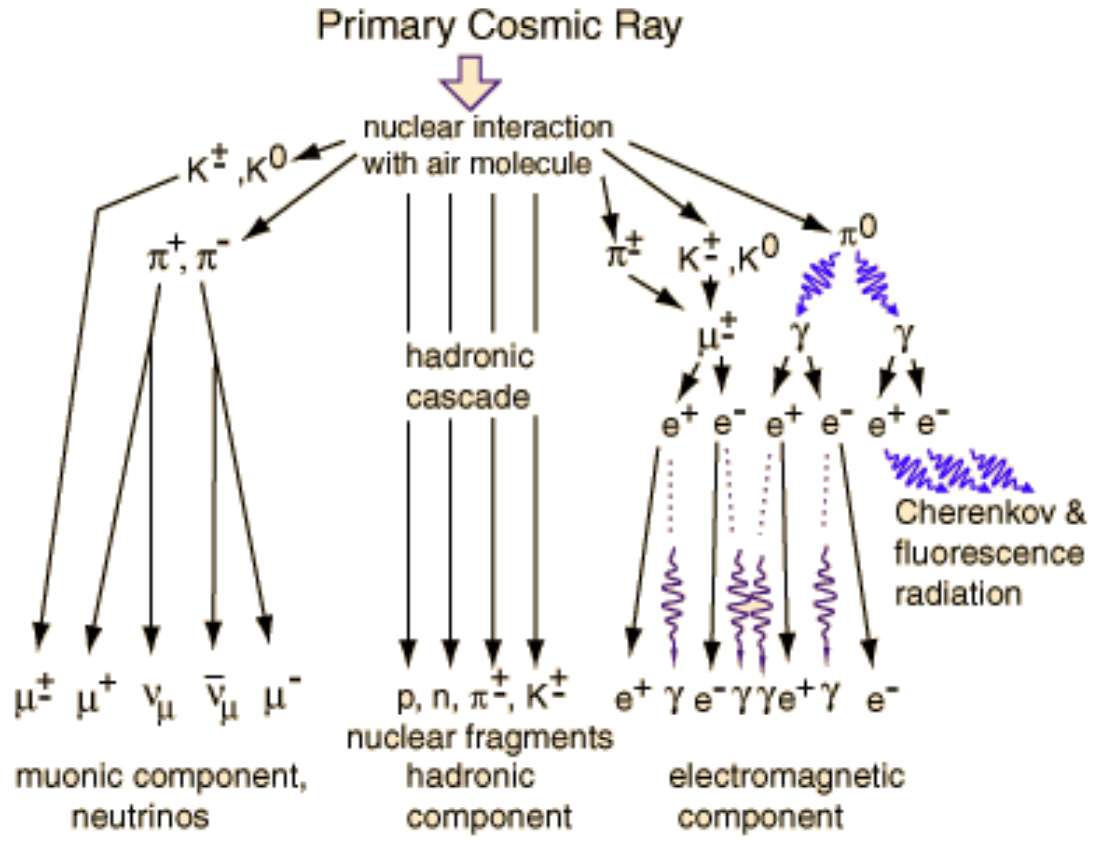
\includegraphics[width=280px]{cara.png}
	\end{figure}
\end{frame}

\begin{frame}{Cherenkov radiation}
	\begin{figure}[h]
		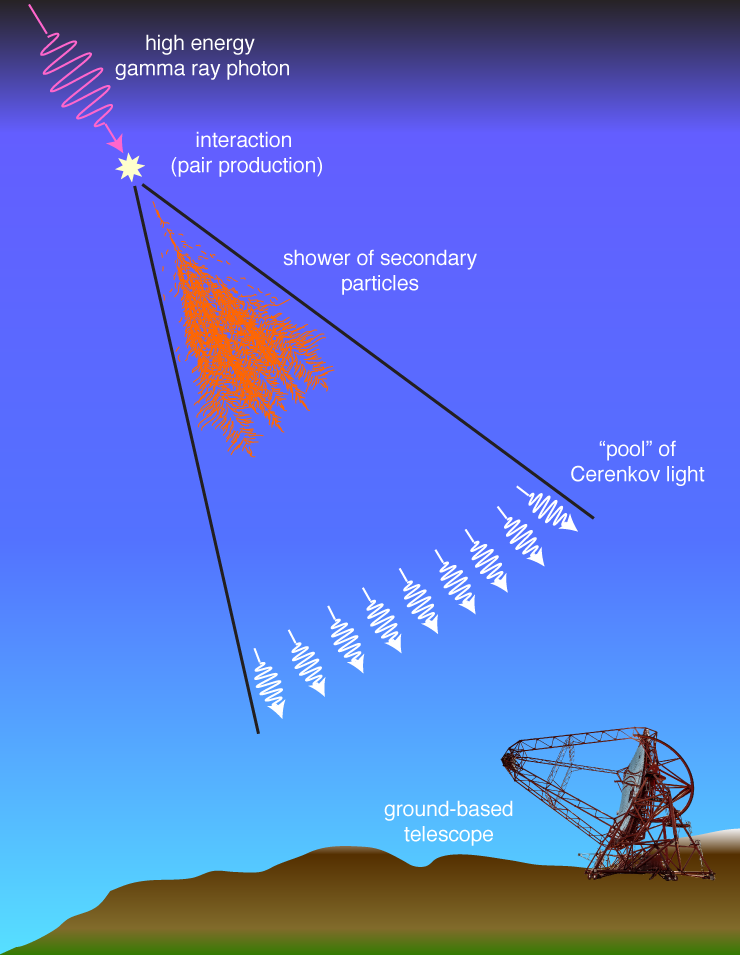
\includegraphics[width=170px]{atmosphere_cerenkov.png}
	\end{figure}
\end{frame}


%%%% Detectors
%%%%%%%%%%%%%%%%%%%%%%%%%%%%%%%%%%%%%%%%%%%%%%%%%%%%%%%%%%%%%
\section{Detectors}
\begin{frame}{Detectors}
	\begin{itemize}
		\item OSO-3 satellite detector
		\item Current ICAT
		\item Future ICAT
	\end{itemize}
\end{frame}



%%%%%%%%%%%%%%%%%%%%%%%%%%%%%%%%%%%%%%%%%%%%%%%%%%%%%%%%%%%%%
\subsection{OSO-3 satellite}
\begin{frame}{OSO-3 satellite}
	OSO 3 (Orbiting Solar Observatory 3)
	\begin{enumerate}
		\item Mar. 8, 1967: launched on
		\item Jun. 28, 1968: tape recorder failed
		\item Nov. 10, 1969: last data were received
		\item Apr. 4, 1982: burned up
	\end{enumerate}
	Result:
	\newline
	The MIT gamma-ray instrument obtained the first identification of high-energy cosmic gamma rays emanating from both galactic and extra-galactic sources
\end{frame}



%%%%%%%%%%%%%%%%%%%%%%%%%%%%%%%%%%%%%%%%%%%%%%%%%%%%%%%%%%%%%
\subsection{Current ICAT}
\begin{frame}{ICAT Properties}
	Properties:
	\begin{enumerate}
		\item 50 GeV $\sim$ 50 TeV in photon energy range
		\item ground-based detector
		\item Wider energy regime than space-based instruments
		\item largest telescope at the highest altitude
		\item work by detecting Cherenkov radiation produced by high energy charged particles
	\end{enumerate}
\end{frame}



\begin{frame}{ICAT components}
	Imaging Atmospheric (or Air) Cherenkov Telescope or Technique
	\newline
	Operating IACT systems:
	\begin{enumerate}
		\item High Energy Stereoscopic System (H.E.S.S.)
		\item Major Atmospheric Gamma Imaging Cherenkov Telescopes (MAGIC)
		\item First G-APD Cherenkov Telescope (FACT)
		\item Very Energetic Radiation Imaging Telescope Array System (VERITAS)
		\item Collaboration of Australia and Nippon for a Gamma Ray Observatory in the Outback (CANGAROO-III)
	\end{enumerate}
	\begin{figure}[h]
		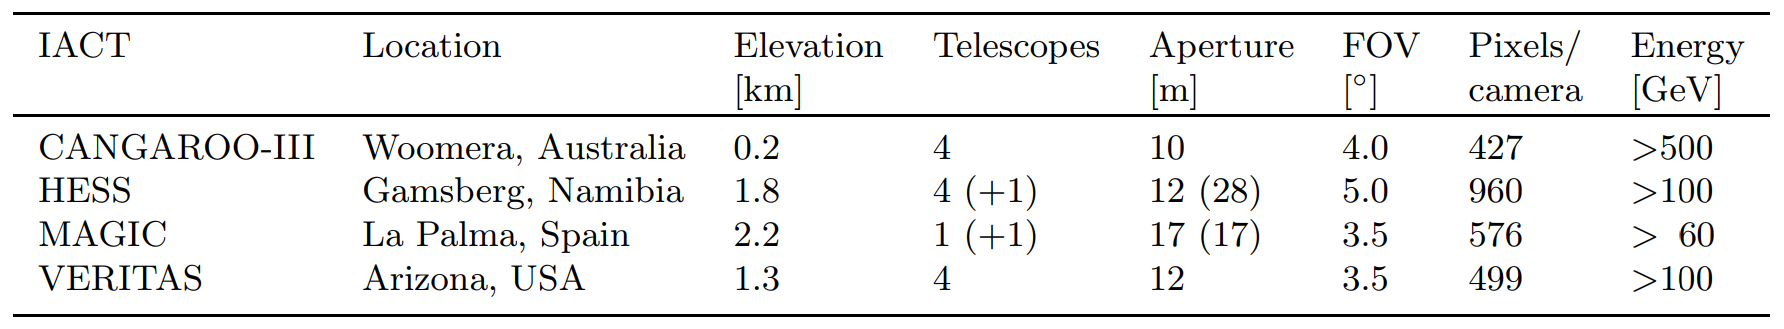
\includegraphics[width=350px]{IACT_tables.png}
	\end{figure}
\end{frame}

\begin{frame}{ICAT components}
	\begin{figure}[h]
		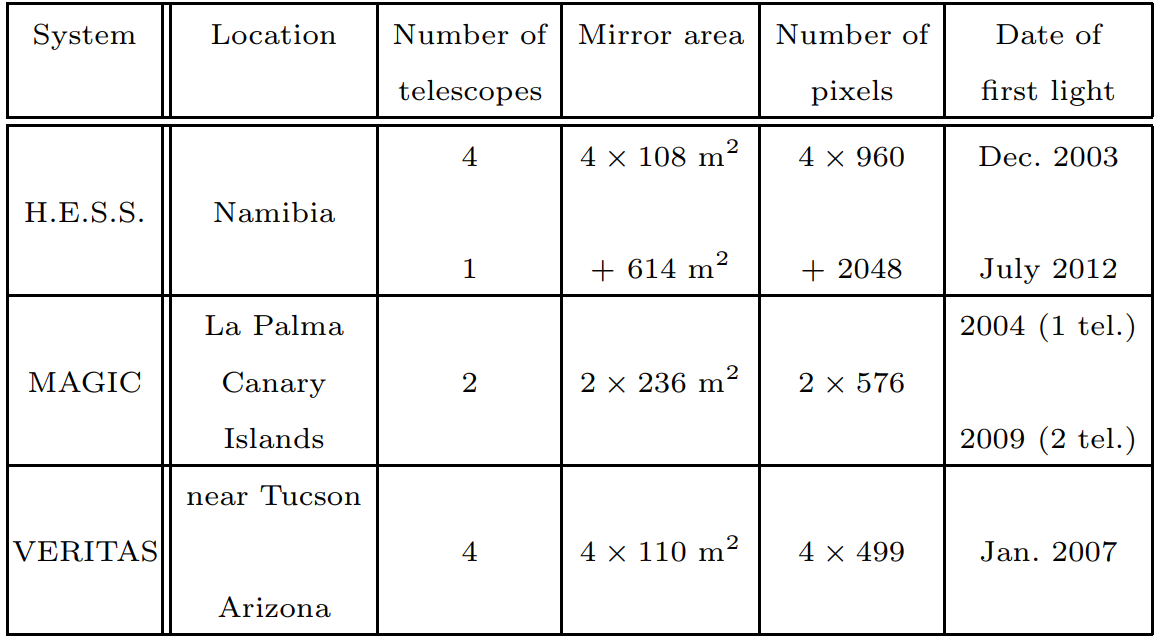
\includegraphics[width=280px]{ICATsystems.png}
	\end{figure}
\end{frame}


\begin{frame}{ICAT components}
	\begin{figure}[h]
		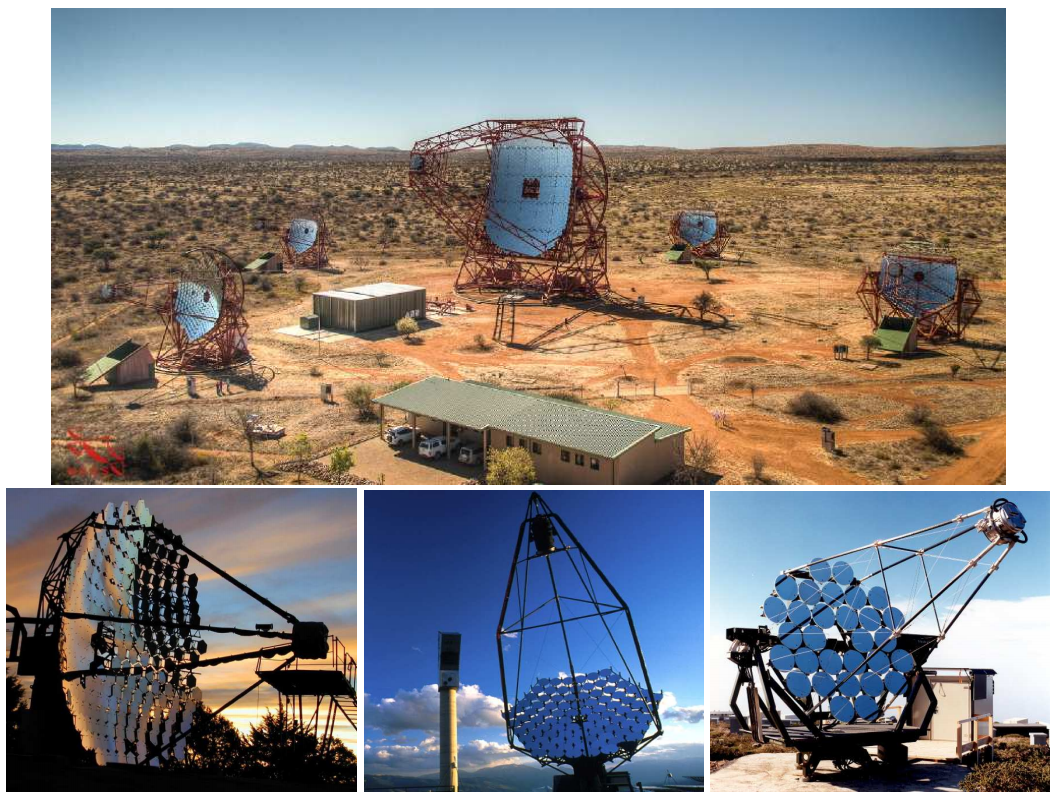
\includegraphics[width=200px]{dishes.png}
		\caption{Illustration of the combination in H.E.S.S. (upper panel) of large dishes as in Whipple (lower left), fast and fine grained cameras as in CAT (lower centre) and stereoscopic observation as in HEGRA (lower right).}
	\end{figure}
\end{frame}


\begin{frame}{ICAT components}
	\begin{figure}[h]
		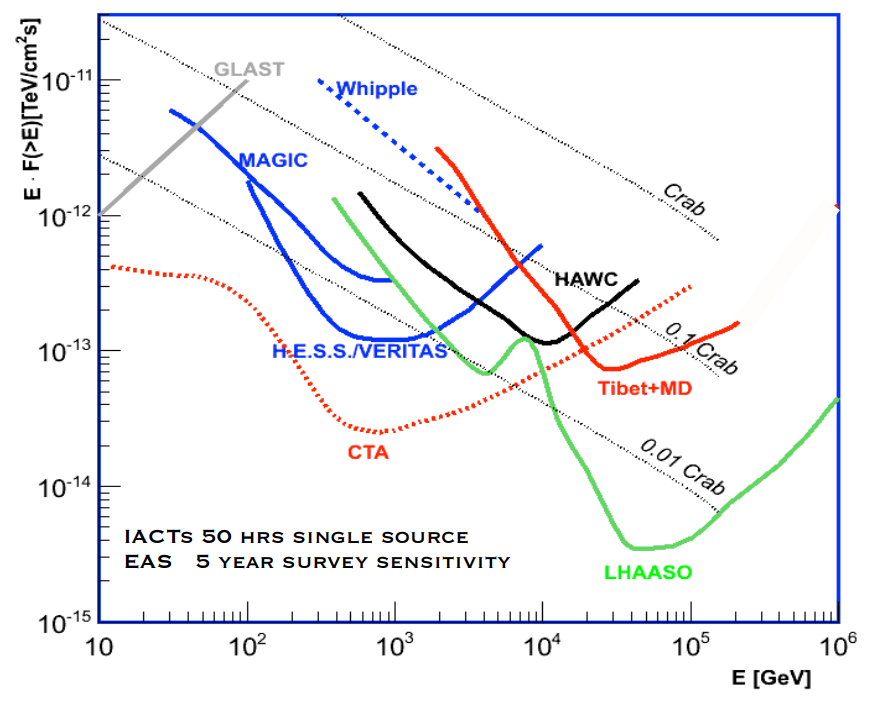
\includegraphics[width=230px]{snesitivities.png}
		\caption{Energy-flux sensitivities of current and future ground-based detectors - the IACT and EAS arrays in the energy range $10^{10}$ to $10^{15}$ eV (courtesy of G. Sinnis).}
	\end{figure}
\end{frame}


%% shown detectors
\begin{frame}{ICAT: FACT}
	G-APD: a new semiconductor device with excellent single photon response became available: the so-called Geiger-mode Avalanche Photodiodes.
	\begin{figure}[h]
		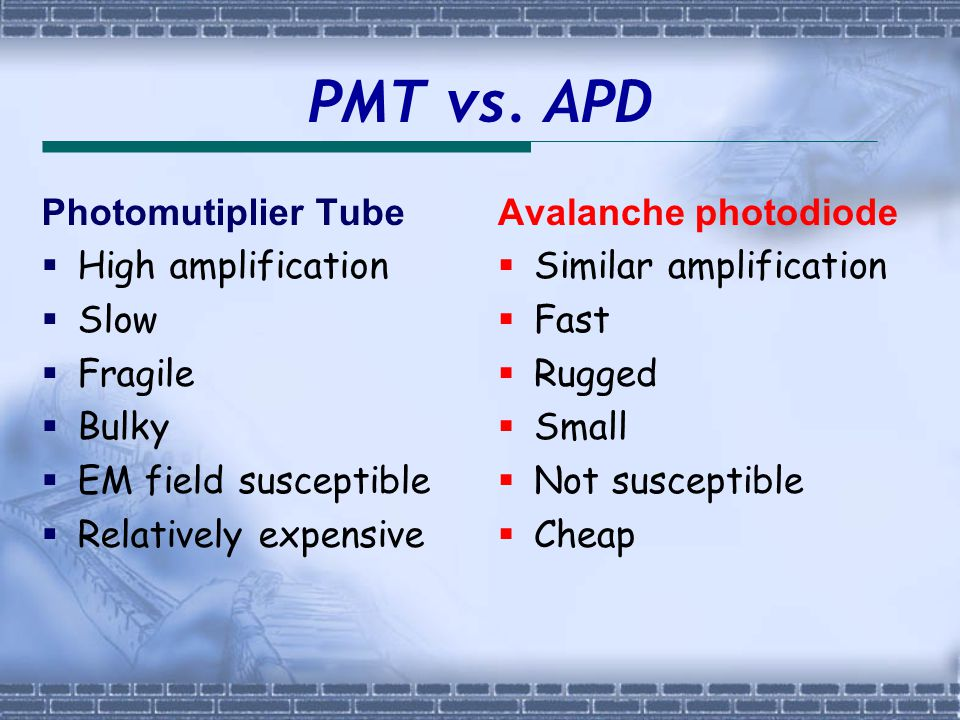
\includegraphics[width=280px]{PMTvsAPD.jpg}
	\end{figure}
\end{frame}


\begin{frame}{ICAT: FACT}
	\begin{figure}[h]
		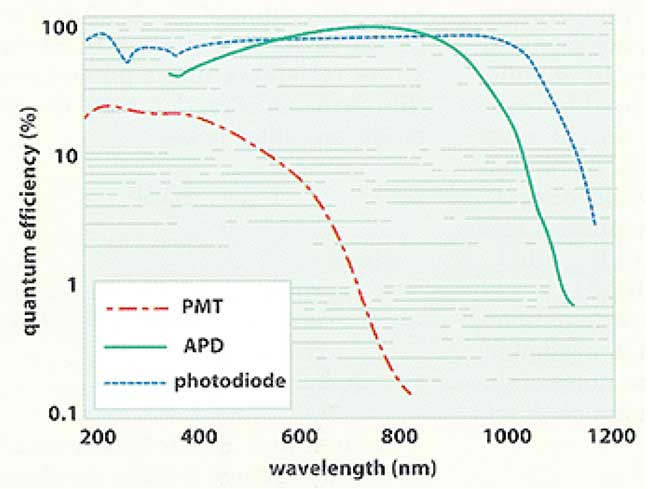
\includegraphics[width=280px]{DetectorsGuidepost.jpg}
	\end{figure}
\end{frame}

% \begin{frame}{ICAT: FACT}
% 	The Photomultiplier (PM) tube
% 	\begin{itemize}
% 		\item Detection of very weak scintillation light
% 		\item Provide electrical signal
% 		\item Can be also done with silicon photodiodes, but PM are most widely used
% 		\item Characterized by spectral sensitivity
% 	\end{itemize}
% \end{frame}


% \begin{frame}{ICAT: FACT}
	% Structure of PM tube
	% \begin{figure}[h]
		% 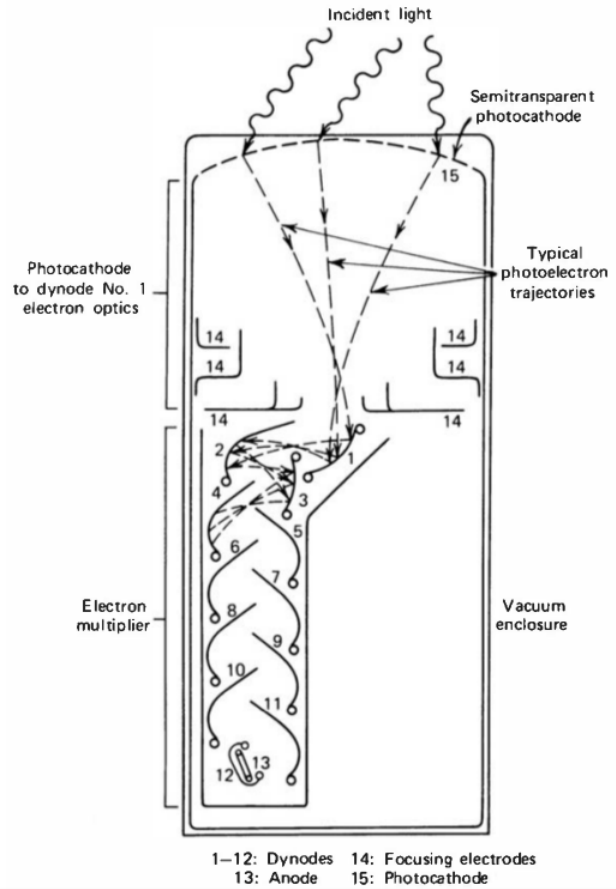
\includegraphics[width=280px]{PM_tube_structure.png}
	% \end{figure}
% \end{frame}


\begin{frame}{ICAT: FACT}
	First G-APD Cherenkov Telescope (FACT), which is based on a former HEGRA telescope.
	\newline
	\\
	Upgrade:
	\begin{itemize}
		\item refurbished mirrors
		\item drive system
	\end{itemize}
\end{frame}


\begin{frame}{ICAT: FACT}
	Mirrors:
	\begin{itemize}
		\item hexagonal shape surface with total area 9.51$m^2$
		\item re-machined by diamond-milling and subsequent coating with \ce{SiO2}.
	\end{itemize}
	\hfill \break
	Drive system:
	\begin{itemize}
		\item down-scaled version of the drive system implemented in the MAGIC telescopes
	\end{itemize}
\end{frame}

\begin{frame}{ICAT: FACT camera}
	\begin{itemize}
		\item 1440 pixels
		\item 4.5 degree FOV
		\item Photo sensors: G-APDs
		\item Solid light guides
	\end{itemize}
	\begin{figure}[h]
		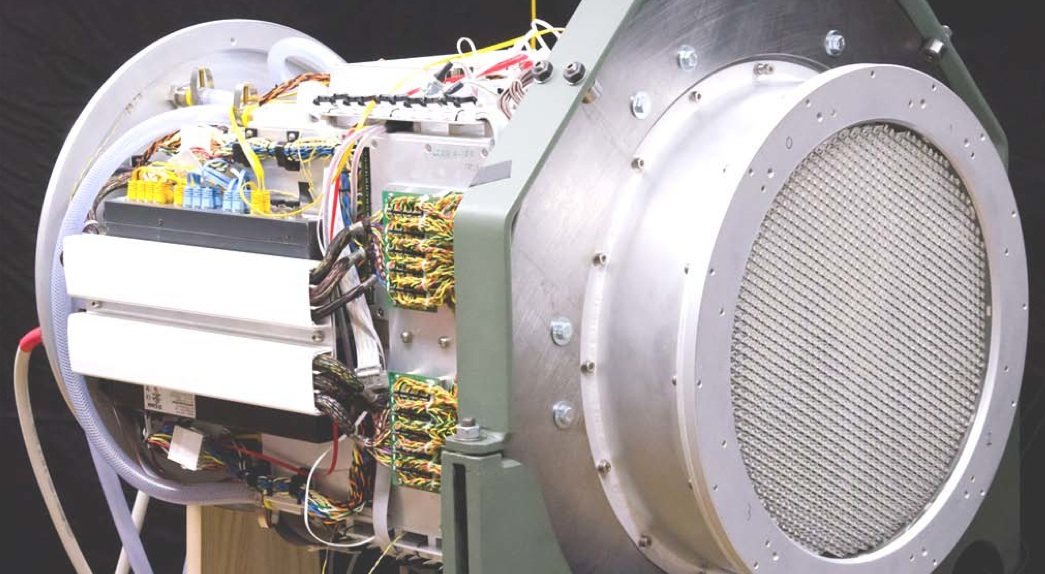
\includegraphics[width=280px]{ICATcamera.jpg}
	\end{figure}
\end{frame}



\begin{frame}{ICAT: FACT telescope}
	\begin{itemize}
		\item Location: 2200 m a.s.l., MAGIC site, Observatorio del Roque de los Muchachos, La Palma, Canary Islands, Spain
		\item Hexagonal mirrors
		\item Mirror area: 9.5 sqm
		\item Energy domain: TeV
	\end{itemize}
	\begin{figure}[h]
		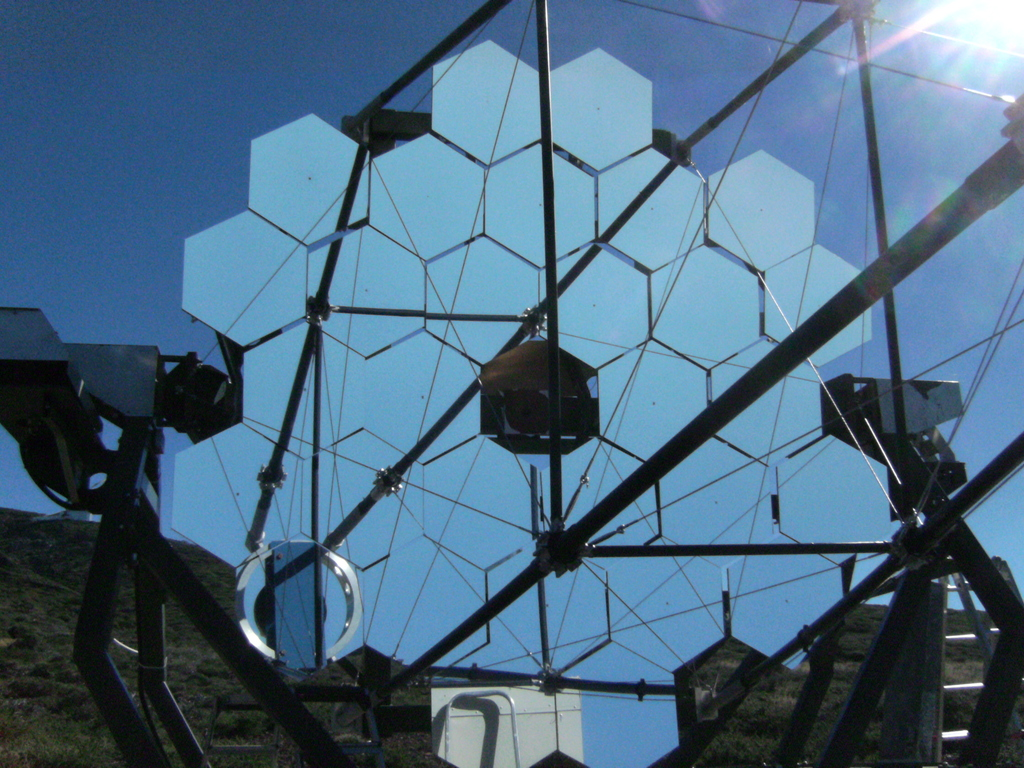
\includegraphics[width=200px]{FACTtelescope.jpg}
	\end{figure}
\end{frame}




\begin{frame}{ICAT: H.E.S.S.}
	High Energy Stereoscopic System (H.E.S.S.)
	\newline
	28 m H.E.S.S. II telescope vs. 12 m H.E.S.S. I telescopes
	\begin{figure}[h]
		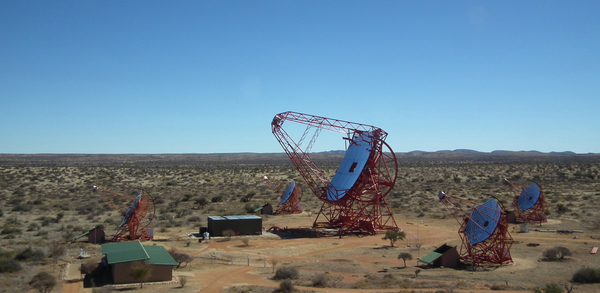
\includegraphics[width=280px]{Array_overviewS.jpg}
	\end{figure}
\end{frame}


\begin{frame}{ICAT: H.E.S.S.}
	Location: 23\textdegree16'18'' S, 16\textdegree30'00'' E at 1800 m
	\newline
	Detection method: Cherenkov technique
	\newline
	Target: gamma ray from Crab Nebula
	\begin{figure}[h]
		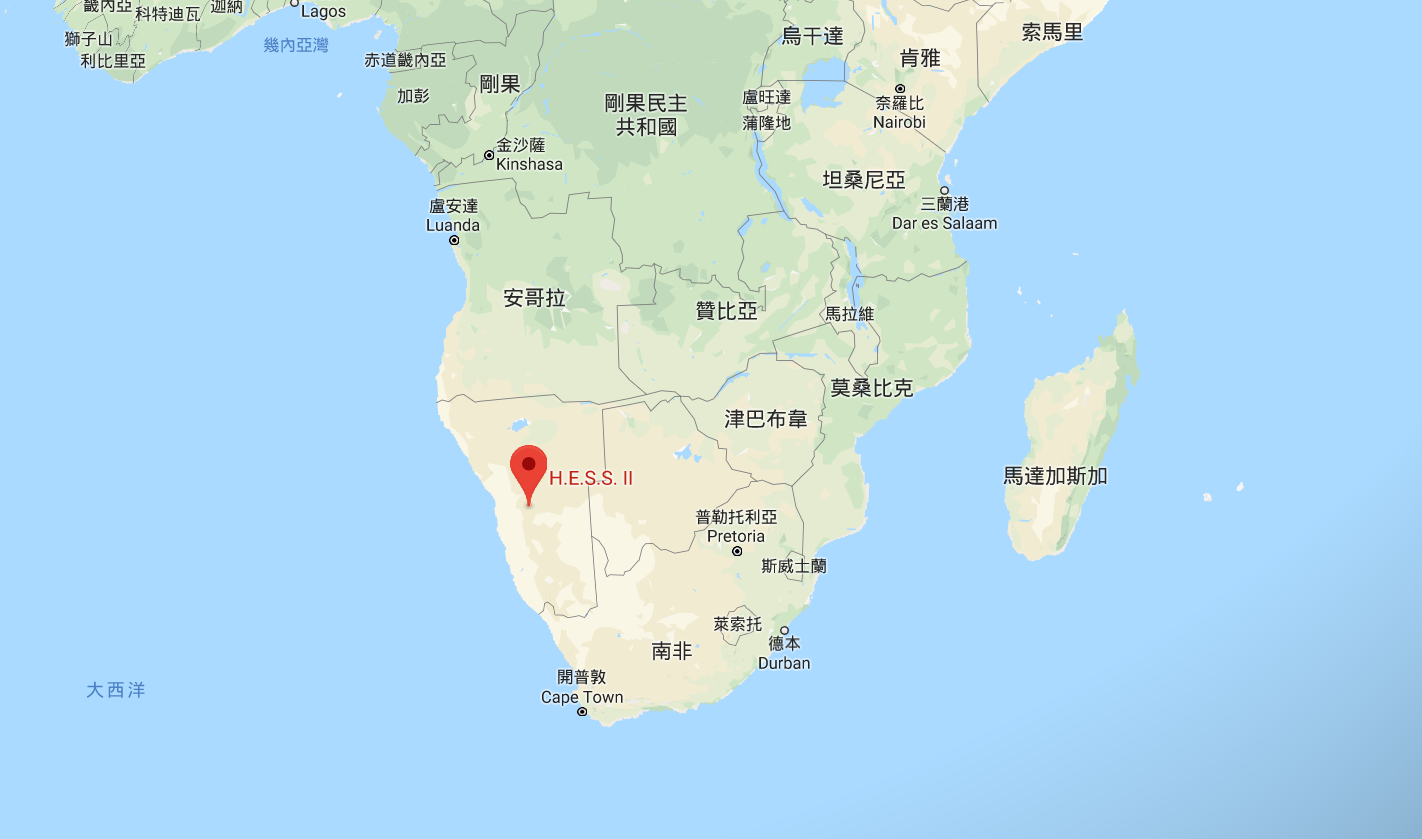
\includegraphics[width=280px]{HESS_location.png}
	\end{figure}
\end{frame}


\begin{frame}{ICAT: H.E.S.S.}
	The H.E.S.S. Collaboration
	\begin{itemize}
		\item 260 scientists
		\item 40 scientific institutions
		\item over 13 different countries
	\end{itemize}
	\begin{figure}[h]
		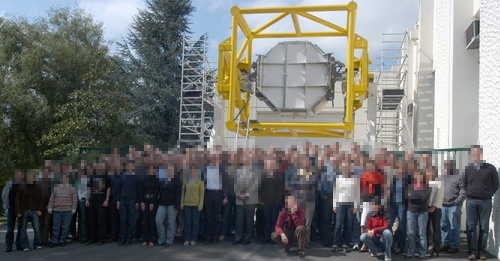
\includegraphics[width=280px]{hess_collaboration.jpg}
	\end{figure}
\end{frame}


\begin{frame}{ICAT: H.E.S.S.}
	Brief history:
	\begin{enumerate}
		\item summer 2002, first operation
		\item Sep 28, 2004, officially inaugurated
		\item 2006, ranked as the 10th most influential observatory worldwide
		\item July 2012, A much larger fifth telescope - H.E.S.S. II installed
		\item Sept. 30, 2012, open day for giant new H.E.S.S. II telescope
		\item 2015-2016, cameras full refurbished
		\item Sep. 27th, 2016, new camera inaugurated
	\end{enumerate}
	\begin{figure}[h]
		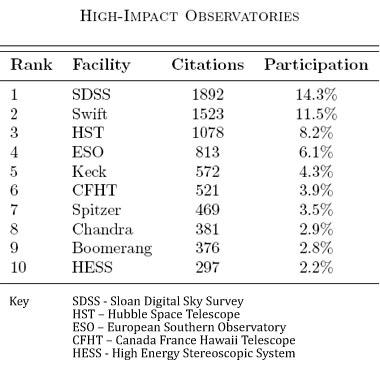
\includegraphics[width=120px]{telescopes-rank.jpg}
	\end{figure}
\end{frame}



\begin{frame}{ICAT: H.E.S.S. telescope}
	Azimuth drive system:
	\begin{itemize}
		\item 12 wheels in 6 bogies on 36 m diameter rail
		\item 4 wheels driven by motors
		\item peak positioning speed 200 degree/minute
		\item range $\pm$ 280 degree
	\end{itemize}
	\hfill \break
	Elevation drive system:
	\begin{itemize}
		\item height of elevation axis: 24 m
		\item 2 drive units with 2 motors each
		\item peak positioning speed 100 degree/minute
		\item range –125 degree +90 degree from vertical
	\end{itemize}
	\hfill \break
	Dish dimensions 32.6 m by 24.3 m ( $\approx$ 28 m circular dish.)
\end{frame}

\begin{frame}{ICAT: H.E.S.S. telescope}
	Elevation drive system
	\, \, \, (the VIDEO)
	\begin{figure}[h]
		\includegraphics[width=280px]{Elevation_Drive_1.JPG}
	\end{figure}
\end{frame}

\begin{frame}{ICAT: H.E.S.S. mirror}
	28 m H.E.S.S. II mirror:
	\begin{itemize}
		\item parabolic shape
		\item Focal length: 36 m
		\item Total mirror area: 614 $m^2$
	\end{itemize}
	\hfill \break
	Mirror facets:
	\begin{itemize}
		\item 875 hexagonal facets of 90 cm (flat-to-flat) size
		\item quartz-coated aluminized glass
		\item weight: 25 kg per facet approx
	\end{itemize}
\end{frame}

\begin{frame}{ICAT: H.E.S.S. mirror}
	Facet alignment: each facet is equipped with 2 actuators with 2 $\mu\text{m}$ positioning step size, corresponding to a 1 arc second facet tilt.
	\begin{figure}[h]
		\includegraphics[width=280px]{2012_mirrors.JPG}
	\end{figure}
\end{frame}


\begin{frame}{ICAT: H.E.S.S. camera}
	The camera of the 28 m telescope:
	\begin{itemize}
		\item Photo sensors: 2048 1-1/4’ photo multipliers
		\item Pixel size: 42 mm (hexagonal, flat-to-flat) $\approx$ 0.067 degree
		\item Sensitive area/field of view: 3.2 degree on the sky
		\item Signal recording: 1 GHz signal sampling; 2 gain channels or each pixel for large dynamic range; records signal amplitude, timing, and shape
		\item Effective signal integration time: 16 ns
		\item Image recording rate: 3600 images/second
		\item Power consumption: 8 kW
		\item Dimensions of camera body: 2.27 wide x 2.4 high x 1.84 deep (meter)
		\item Camera weight: 2.8 tons
		\item Camera support: Quadrupod
	\end{itemize}
\end{frame}




\begin{frame}{ICAT: MAGIC}
	Major Atmospheric Gamma Imaging Cherenkov Telescopes (MAGIC)
\end{frame}


\begin{frame}{ICAT: VERITAS}
	Very Energetic Radiation Imaging Telescope Array System (VERITAS)
\end{frame}


\begin{frame}{ICAT: CANGAROO-III}
	CANGAROO-III (Collaboration of Australia and Nippon for a Gamma Ray Observatory in the Outback)
\end{frame}

%%%%%%%%%%%%%%%%%%%%%%%%%%%%%%%%%%%%%%%%%%%%%%%%%%%%%%%%%%%%%
\subsection{Future ICAT}
\begin{frame}{Future ICAT improvement}
	Improvement:
	\begin{enumerate}
		\item enhance flux sensitivities in TeV regime (0.1-10 TeV)
		\item expand energy domain: down to 10 GeV (multi-GeV regime) and well beyond 10 TeV (sub-PeV regime)
	\end{enumerate}
\end{frame}


\begin{frame}{Future ICAT: TeV regime}
	\begin{enumerate}
		\item minimum detectable energy flux: $10$ erg$/ \text{cm}^2 $ s
		\item angular resolution: $\delta \theta \leq 3$ arc minutes.
	\end{enumerate}
\end{frame}


\begin{frame}{Next generation CTA}
	\begin{figure}[h]
		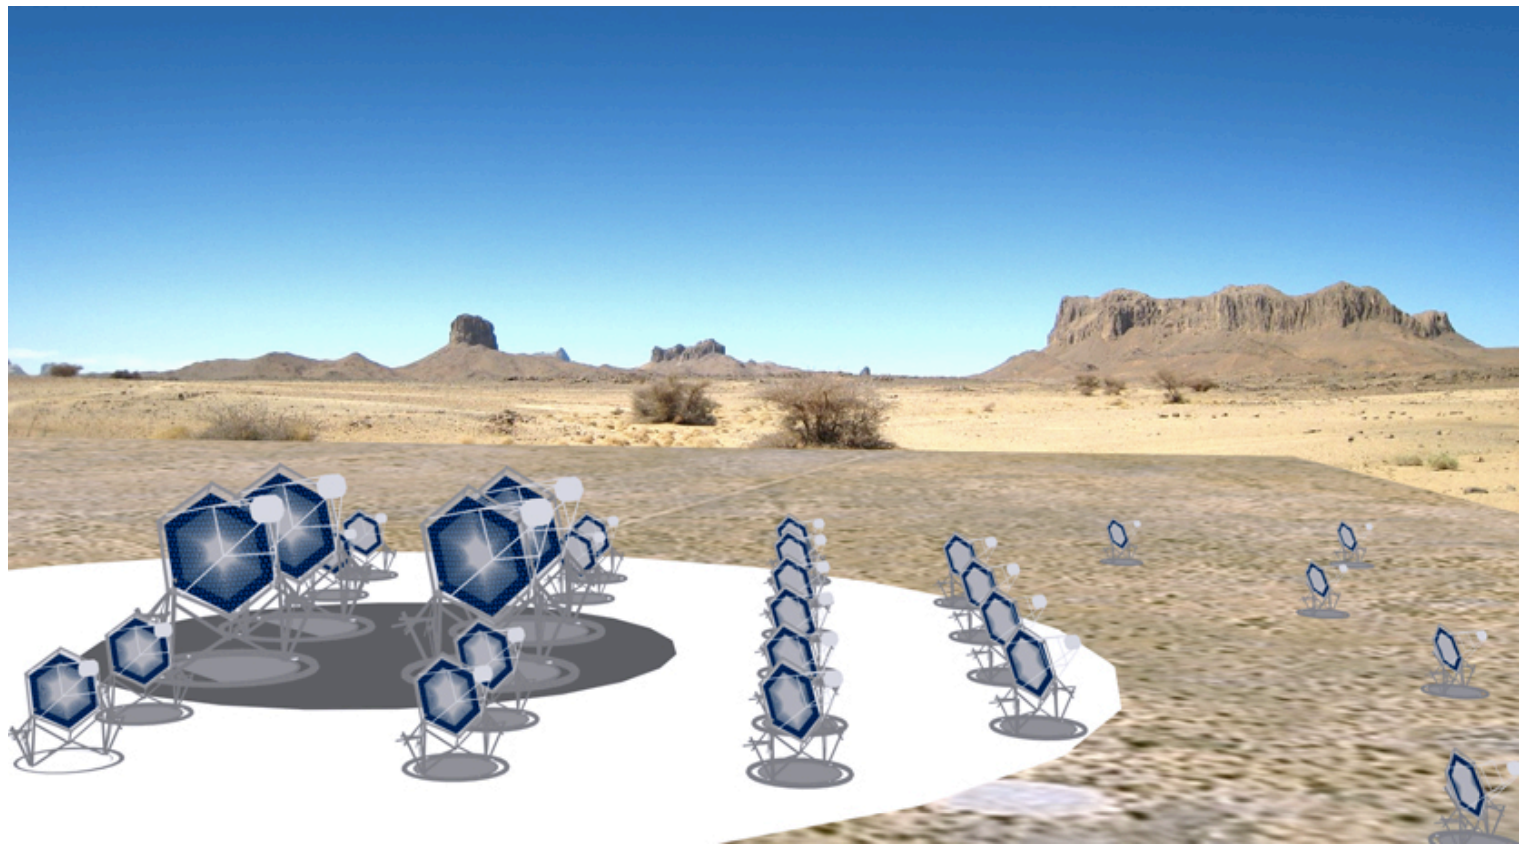
\includegraphics[width=300px]{next-generationCTA.png}
		\caption{Possible layout of the next-generation CTA instrument}
	\end{figure}
\end{frame}




\end{document}